\section{eo\-Bit\-Gx\-Over$<$ Chrom $>$ Class Template Reference}
\label{classeo_bit_gx_over}\index{eoBitGxOver@{eoBitGxOver}}
eo\-Bit\-Gx\-Over --$>$ Npts crossover when bistd::string considered as a std::string of binary-encoded genes (exchanges genes) Is anybody still using it apart from historians ??? :-)  


{\tt \#include $<$ga/eo\-Bit\-Op.h$>$}

Inheritance diagram for eo\-Bit\-Gx\-Over$<$ Chrom $>$::\begin{figure}[H]
\begin{center}
\leavevmode
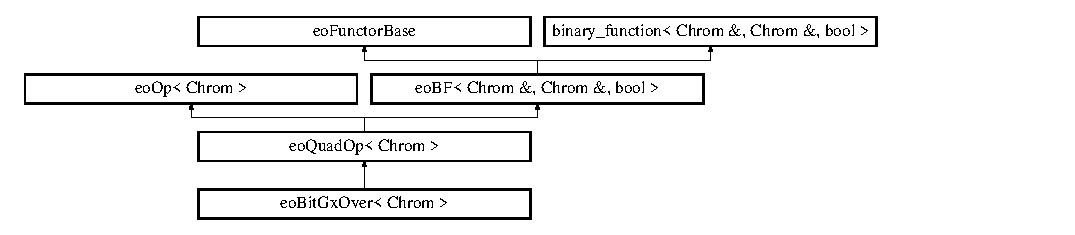
\includegraphics[height=2.70531cm]{classeo_bit_gx_over}
\end{center}
\end{figure}
\subsection*{Public Member Functions}
\begin{CompactItemize}
\item 
{\bf eo\-Bit\-Gx\-Over} (const unsigned \_\-gene\_\-size, const unsigned \_\-num\_\-points=2)\label{classeo_bit_gx_over_a0}

\begin{CompactList}\small\item\em Constructor. \item\end{CompactList}\item 
virtual std::string {\bf class\-Name} () const \label{classeo_bit_gx_over_a1}

\begin{CompactList}\small\item\em The class name. \item\end{CompactList}\item 
bool {\bf operator()} (Chrom \&chrom1, Chrom \&chrom2)
\begin{CompactList}\small\item\em Gene crossover for binary chromosomes. \item\end{CompactList}\end{CompactItemize}
\subsection*{Private Attributes}
\begin{CompactItemize}
\item 
unsigned {\bf gene\_\-size}\label{classeo_bit_gx_over_r0}

\item 
unsigned {\bf num\_\-points}\label{classeo_bit_gx_over_r1}

\end{CompactItemize}


\subsection{Detailed Description}
\subsubsection*{template$<$class Chrom$>$ class eo\-Bit\-Gx\-Over$<$ Chrom $>$}

eo\-Bit\-Gx\-Over --$>$ Npts crossover when bistd::string considered as a std::string of binary-encoded genes (exchanges genes) Is anybody still using it apart from historians ??? :-) 



Definition at line 388 of file eo\-Bit\-Op.h.

\subsection{Member Function Documentation}
\index{eoBitGxOver@{eo\-Bit\-Gx\-Over}!operator()@{operator()}}
\index{operator()@{operator()}!eoBitGxOver@{eo\-Bit\-Gx\-Over}}
\subsubsection{\setlength{\rightskip}{0pt plus 5cm}template$<$class Chrom$>$ bool {\bf eo\-Bit\-Gx\-Over}$<$ Chrom $>$::operator() (Chrom \& {\em chrom1}, Chrom \& {\em chrom2})\hspace{0.3cm}{\tt  [inline, virtual]}}\label{classeo_bit_gx_over_a2}


Gene crossover for binary chromosomes. 

\begin{Desc}
\item[Parameters:]
\begin{description}
\item[{\em chrom1}]The first chromosome. \item[{\em chrom2}]The first chromosome. \end{description}
\end{Desc}


Implements {\bf eo\-BF$<$ Chrom \&, Chrom \&, bool $>$} {\rm (p.\,\pageref{classeo_b_f_a1})}.

Definition at line 409 of file eo\-Bit\-Op.h.

The documentation for this class was generated from the following file:\begin{CompactItemize}
\item 
eo\-Bit\-Op.h\end{CompactItemize}
